\documentclass[tikz,border=3mm]{standalone}
\usepackage{tikz}
\usepackage{amsmath}
\begin{document}
	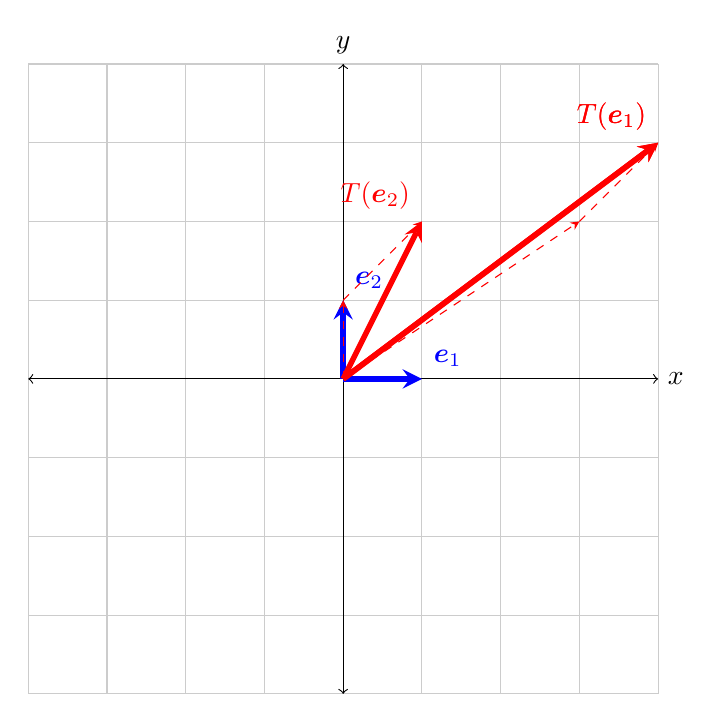
\begin{tikzpicture}
		\draw[thin,gray!40] (-4,-4) grid (4,4);
		\draw[<->] (-4,0)--(4,0) node[right]{$x$};
		\draw[<->] (0,-4)--(0,4) node[above]{$y$};
		\draw[line width=2pt,blue,-stealth](0,0)--(1,0) node[anchor=south west]{$\boldsymbol{e}_1$};
		\draw[line width=2pt,red,-stealth](0,0)--(4,3) node[anchor=south east]{$T(\boldsymbol{e}_1)$};
		\draw[dashed ,red,-stealth](0,0)--(3,2);
		\draw[dashed,red,-stealth](3,2)--(4,3);
		\draw[line width=2pt,red,-stealth](0,0)--(4,3) node[anchor=south east]{$T(\boldsymbol{e}_1)$};
		\draw[line width=2pt,blue,-stealth](0,0)--(0,1) node[anchor=south west]{$\boldsymbol{e}_2$};
		\draw[dashed ,red,-stealth](0,0)--(0,1);
		\draw[dashed,red,-stealth](0,1)--(1,2);
		\draw[line width=2pt,red,-stealth](0,0)--(1,2) node[anchor=south east]{$T(\boldsymbol{e}_2)$};
	\end{tikzpicture}
\end{document}